\chapter{Implementation}
\label{ch:implementation}

\section{Technology stack and interface}

The backend uses Python, FastAPI, SQLModel, Pydantic settings, SQLite, and PyMuPDF. The frontend uses React, TypeScript, and Vite. Eight views expose dashboard statistics, papers, search, Ask TTLAB, extension recommendations, topic/author exploration, administrative review, and evaluation. \Cref{fig:dashboard-shot,fig:search-shot} show the audited runtime.

\begin{figure}[htbp]
\centering
\projectScreenshot{figures/screenshots/dashboard.png}{0.96\textwidth}
\caption{Dashboard in the audited browser session. The empty top-topic widget contrasts with populated explorer data and is retained as failure evidence.}
\label{fig:dashboard-shot}
\end{figure}

\begin{figure}[htbp]
\centering

\includegraphics[width=0.96\textwidth,trim=0 950bp 0 0,clip]{figures/screenshots/search-results.png}
\caption{Search results with mode, scores, paper metadata, pages, and source snippets. The full-page capture is deliberately cropped to its top results for legibility.}
\label{fig:search-shot}
\end{figure}

Navigation is held in React state rather than URL routes, so refreshing returns to the dashboard and views are not deep-linkable.

\section{Keyword and hashing-vector retrieval}

SQLite FTS5 indexes all chunk text and returns its \texttt{bm25()} rank, transformed by
\begin{equation}
K = \frac{1}{1+|r_{\mathrm{FTS}}|}.
\label{eq:fts-transform}
\end{equation}
A deterministic fallback combines term frequency and query coverage when FTS is unavailable.

The vector path maps token $t$ into one of $d=256$ coordinates and a sign using SHA-256. For document $x$, the unnormalised coordinate is
\begin{equation}
z_j(x)=\sum_{t\in x}\mathbb{I}[h(t)=j]s(t), \qquad
\mathbf{v}(x)=\frac{\mathbf{z}(x)}{\lVert\mathbf{z}(x)\rVert_2}.
\label{eq:hashing}
\end{equation}
Similarity is the dot product $V=\mathbf{v}(q)^\top\mathbf{v}(c)$, equivalent to cosine similarity after normalisation. This is feature hashing \cite{weinberger2009featurehashing}, not a learned semantic encoder.

\section{Hybrid scoring and diversification}

Current working-tree code removes a fixed stop-word set, applies fixed domain query expansions, and computes
\begin{equation}
H=\operatorname{clip}_{[0,1]}(0.42K+0.48V+M+S+E+T),
\label{eq:hybrid}
\end{equation}
where $M$ is metadata match, $S$ an intent-dependent section boost, $E$ an evidence-quality adjustment, and $T$ topical alignment. A greedy penalty reduces repeated or adjacent chunks from the same paper. The coefficients are hand-authored; no tuning or ablation evidence exists.

\section{Question answering}

The workflow in \cref{fig:rag-workflow} retrieves chunks, composes an answer with a deterministic offline provider or local Ollama, attaches citations, verifies structural properties, persists the result, and displays the answer with source pages and warnings.

\begin{figure}[htbp]
\centering
\begingroup\hfuzz=100pt\resizebox{\textwidth}{!}{\begingroup\hfuzz=100pt
\begin{tikzpicture}[node distance=8mm and 9mm]
  \node[flowbox] (question) {Question + retrieval mode,\\top-$k$, audience, paper filter};
  \node[flowbox, right=of question] (prepare) {Stop-word handling +\\fixed expansion when enabled};
  \node[flowbox, right=of prepare] (retrieve) {Keyword FTS, 256-d hashing,\\384-d pinned dense, or hybrid};
  \node[flowbox, right=of retrieve] (rerank) {Optional metadata, section, evidence,\\topic and diversity adjustments};

  \node[datastore, below=14mm of retrieve] (chunks) {Scope-filtered chunks\\paper, page, section, hash};
  \node[decision, left=12mm of chunks] (provider) {Evidence\\answerable?};
  \node[flowbox, left=12mm of provider] (compose) {Offline extractive or\\local Ollama composition};
  \node[flowbox, left=of compose] (cite) {Return answer plus citations,\\snippets and retrieved chunks};

  \node[flowbox, below=14mm of cite] (verify) {Structural locator/membership check;\\later atomic AI-silver review};
  \node[decision, right=of verify] (status) {Grounding /\\warning state};
  \node[datastore, right=of status] (persist) {Transient by default;\\protected history/review};
  \node[flowbox, right=of persist] (display) {Evidence, provider/time, review state,\\unsupported/partial warnings};

  \draw[arrow] (question) -- (prepare);
  \draw[arrow] (prepare) -- (retrieve);
  \draw[arrow] (retrieve) -- (rerank);
  \draw[arrow] (rerank) -- (chunks);
  \draw[arrow] (chunks) -- (provider);
  \draw[arrow] (provider) -- (compose);
  \draw[arrow] (compose) -- (cite);
  \draw[arrow] (cite) -- (verify);
  \draw[arrow] (verify) -- (status);
  \draw[arrow] (status) -- (persist);
  \draw[arrow] (persist) -- (display);
  \draw[dashedarrow] (provider.south) -- ++(0,-6mm) node[below,font=\scriptsize,align=center]{Insufficient coverage abstains; provider failure\\is explicit and may fall back to extraction};
\end{tikzpicture}
\endgroup
}\endgroup
\caption{Implemented search and RAG workflow. The verifier checks structure, membership, and lexical overlap rather than semantic entailment.}
\label{fig:rag-workflow}
\end{figure}

The Ollama adapter uses a low-temperature, source-restricted prompt and falls back on error. The OpenAI provider branch raises a not-implemented error. The verifier requires retrieved chunks, complete citation fields, citation membership, and at least 0.08 answer-to-snippet token overlap. Therefore, its \texttt{grounded} label means structurally/lexically grounded only.

\begin{figure}[htbp]
\centering
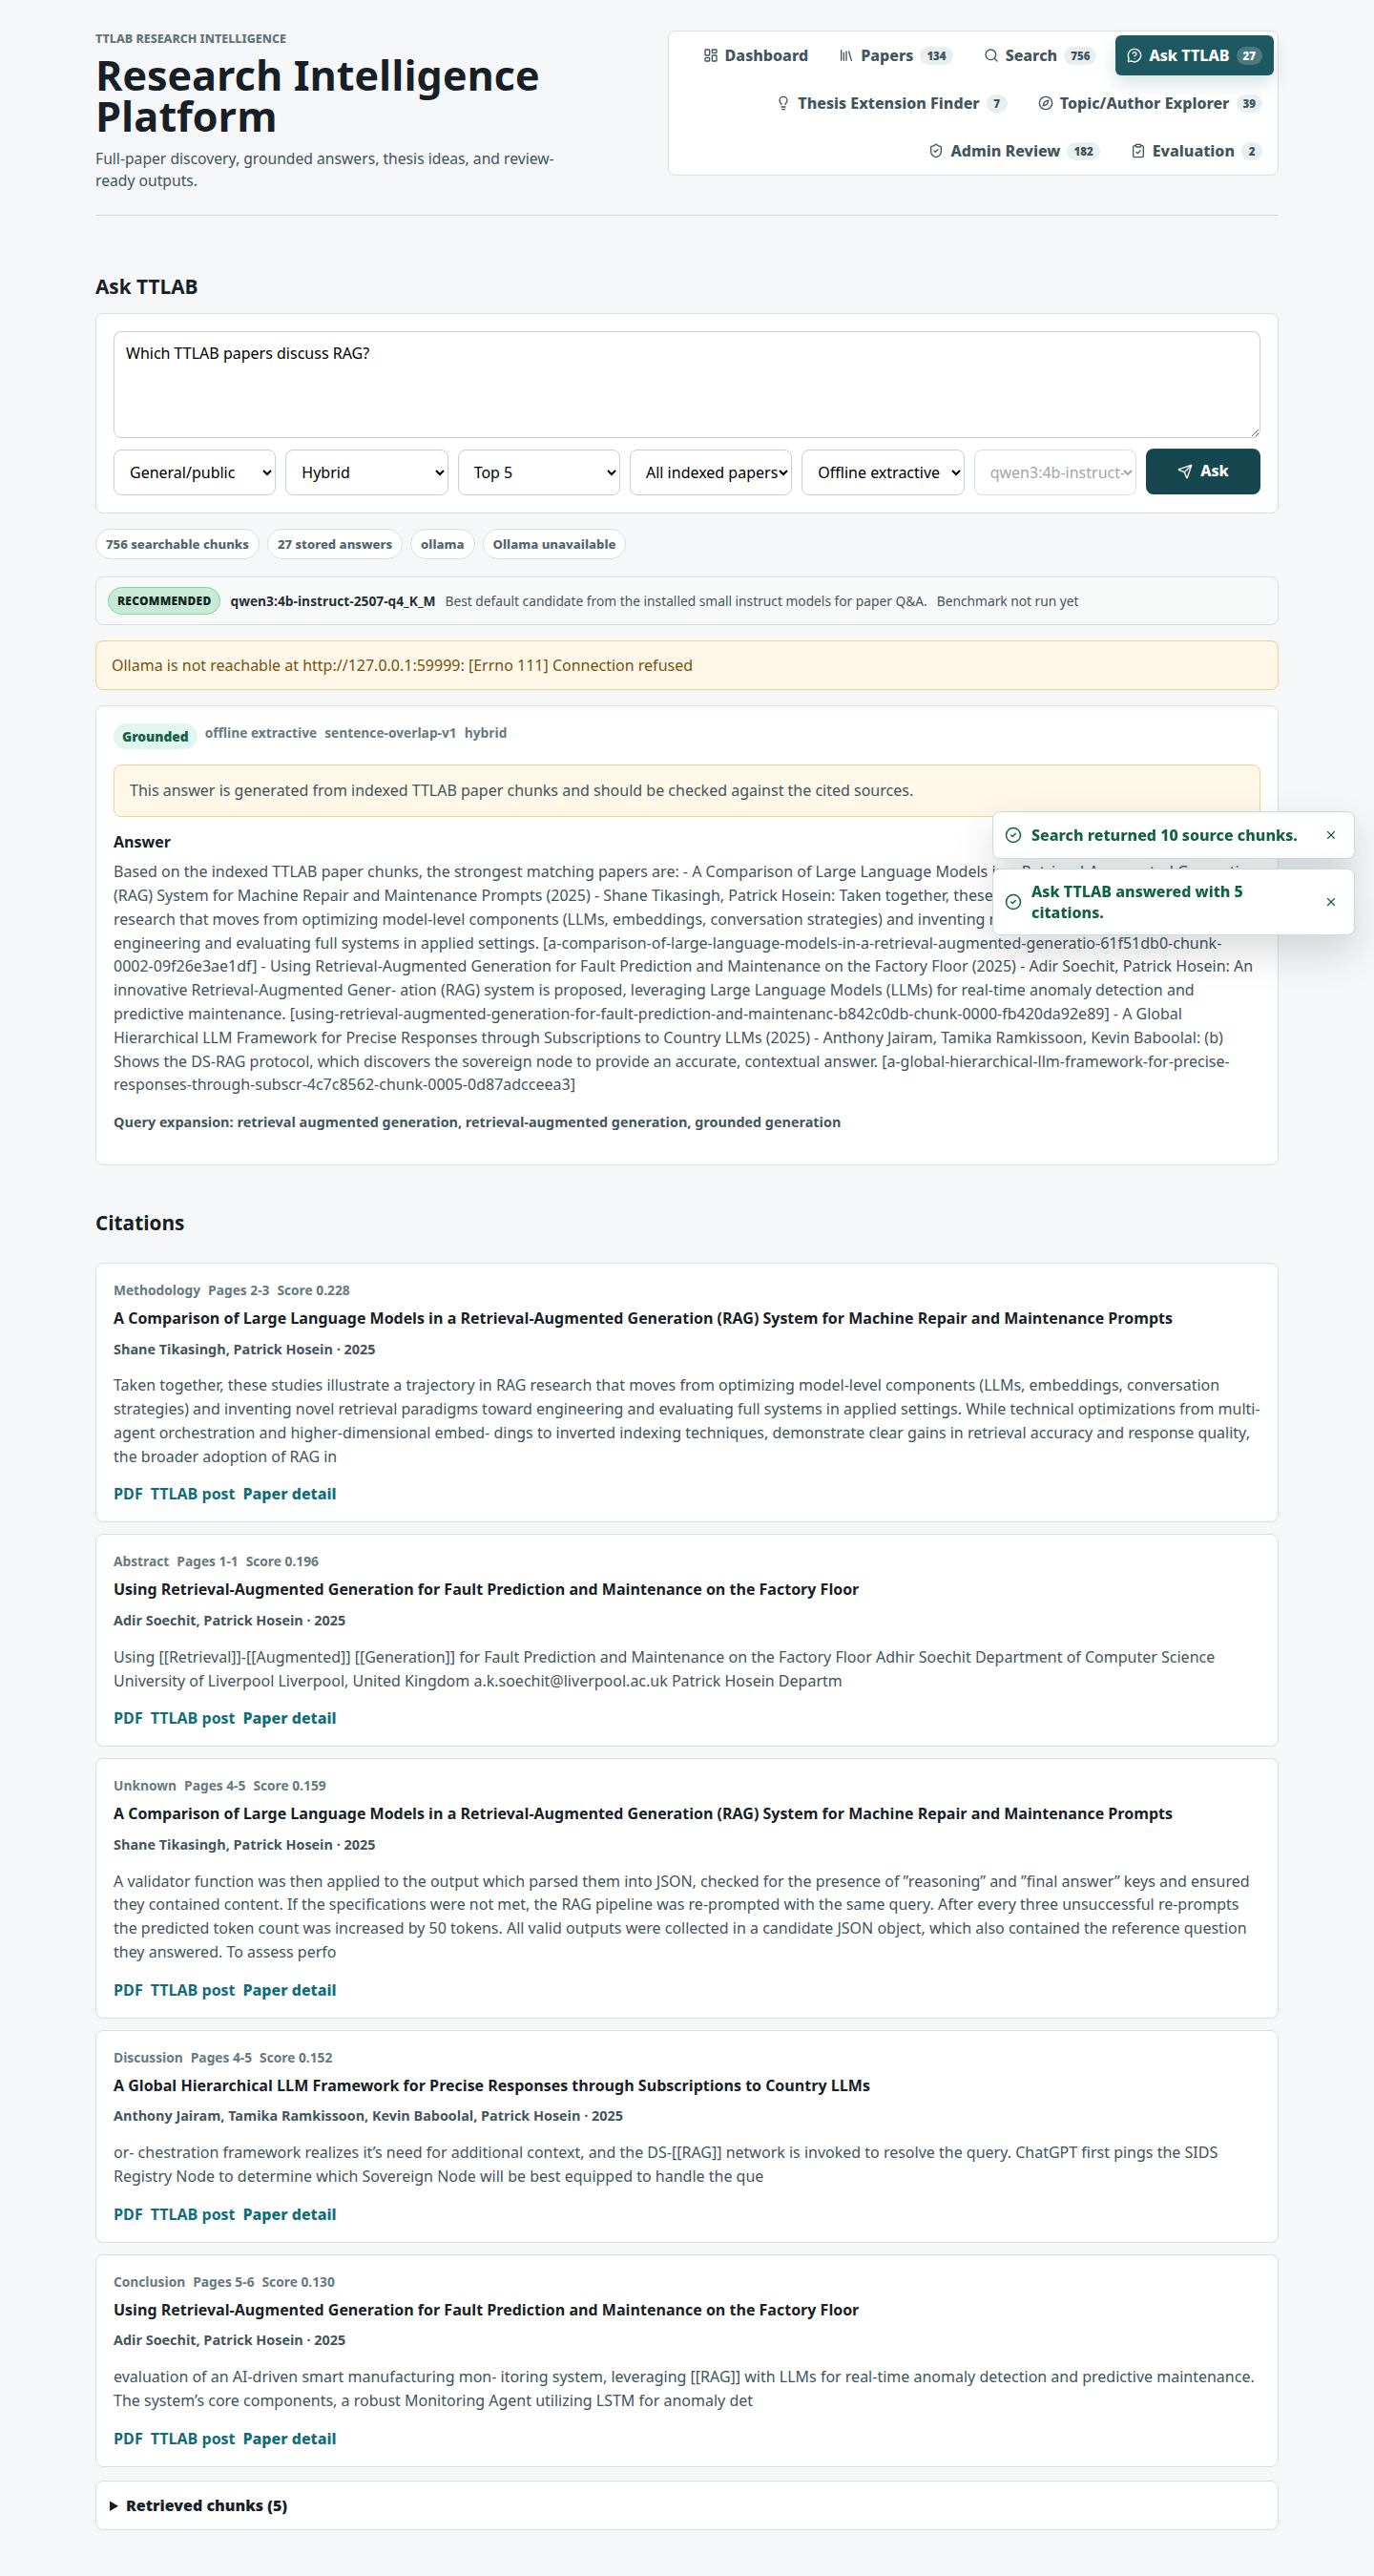
\includegraphics[width=0.96\textwidth,trim=0 900bp 0 0,clip]{figures/screenshots/ask-answer.png}
\caption{Ask TTLAB response showing generated-answer notice, grounding state, and cited papers. The full-page capture is deliberately cropped to the answer and leading citations.}
\label{fig:ask-shot}
\end{figure}

\section{Thesis-extension recommendations}

\Cref{fig:recommendation-workflow} shows the deterministic workflow. Candidate paper score $R$ is
\begin{align}
R={}&0.30r+0.20i+0.15s+0.10d+0.10t \\
   &+0.10f+0.05e-0.20a,
\label{eq:recommendation}
\end{align}
where the terms represent retrieval relevance, interest, skill, data, time, difficulty fit, evidence strength, and avoided-topic match. The output distinguishes an explicit, inferred, or absent source gap from the system's suggested extension.

\begin{figure}[htbp]
\centering
\begingroup\hfuzz=100pt\resizebox{\textwidth}{!}{\begingroup\hfuzz=100pt
\begin{tikzpicture}[node distance=8mm and 9mm]
  \node[flowbox] (profile) {Student profile\\interests, skills, time, type,\\data, difficulty, avoid topics};
  \node[flowbox, right=of profile] (query) {Build retrieval query +\\future-work terms};
  \node[flowbox, right=of query] (retrieve) {Retrieve up to\\$6\times k$ chunks};
  \node[flowbox, right=of retrieve] (group) {Group evidence by paper};

  \node[flowbox, below=15mm of group] (score) {Weighted score: relevance .30;\\interest .20; skill .15;\\data/time/difficulty .10 each;\\evidence .05; avoid $-.20$};
  \node[flowbox, left=of score] (gap) {Detect explicit, inferred,\\or missing gap evidence};
  \node[flowbox, left=of gap] (draft) {Template suggestion, MVP,\\stretch goals, skills, risk,\\data and evaluation plan};
  \node[flowbox, left=of draft] (verify) {Check citation membership,\\gap status and warnings};

  \node[datastore, text width=28mm, below=15mm of verify] (persist) {Thesis\\Recommendation\\partial, grounded,\\unsupported; needs review};
  \node[flowbox, right=of persist] (ui) {Ranked, cited output or\\evidence-only paper/passages};
  \node[flowbox, right=of ui, fill=PaleTeal, draw=Teal!80!black] (proxy) {Paired AI-proxy review\\with source rationales};

  \draw[arrow] (profile) -- (query);
  \draw[arrow] (query) -- (retrieve);
  \draw[arrow] (retrieve) -- (group);
  \draw[arrow] (group) -- (score);
  \draw[arrow] (score) -- (gap);
  \draw[arrow] (gap) -- (draft);
  \draw[arrow] (draft) -- (verify);
  \draw[arrow] (verify) -- (persist);
  \draw[arrow] (persist) -- (ui);
  \draw[arrow] (ui) -- (proxy);
\end{tikzpicture}
\endgroup
}\endgroup
\caption{Implemented recommendation pipeline and the human-validation stage that has not yet been executed.}
\label{fig:recommendation-workflow}
\end{figure}

\begin{figure}[htbp]
\centering
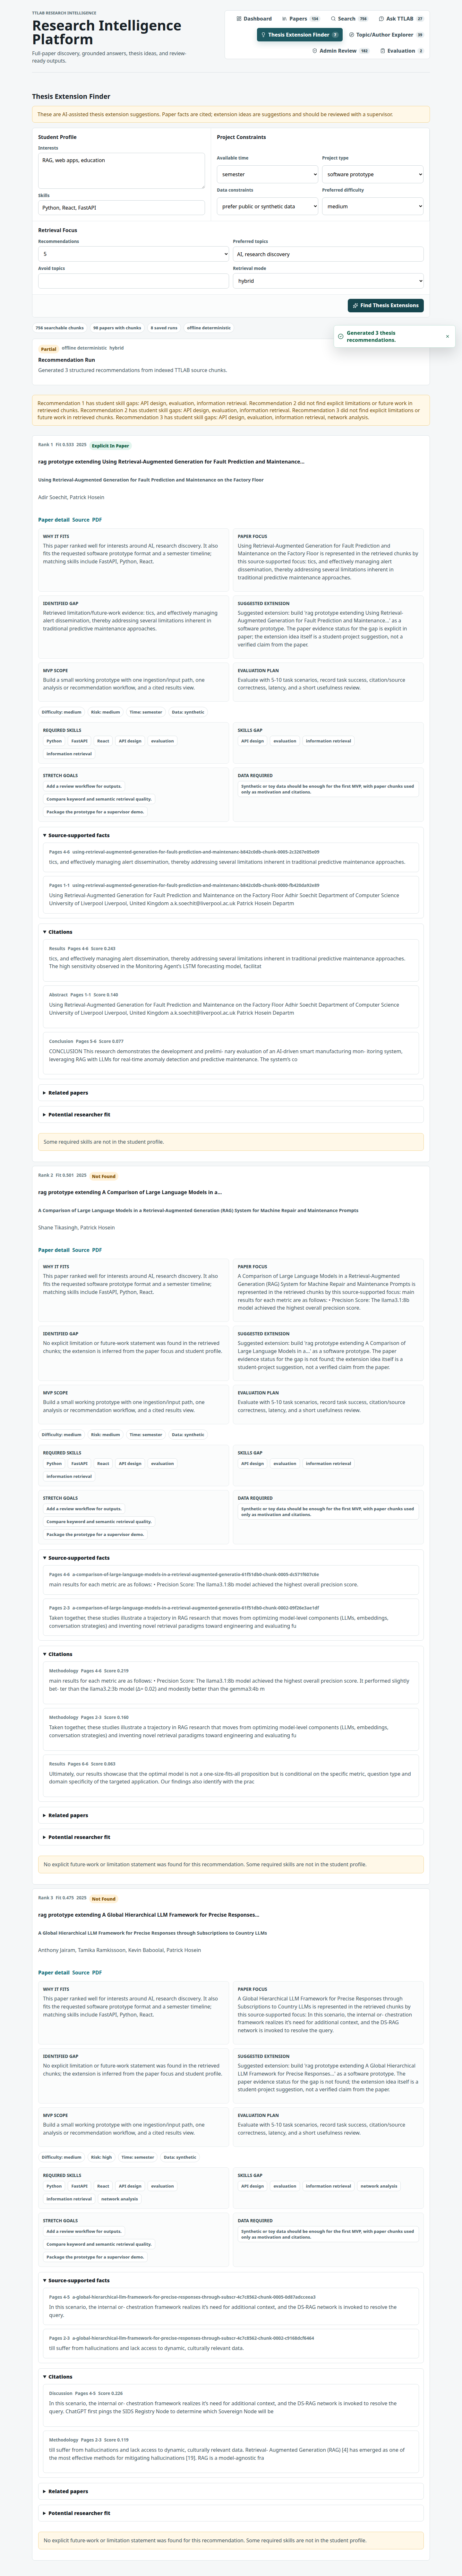
\includegraphics[width=0.96\textwidth,trim=0 6500bp 0 0,clip]{figures/screenshots/extension-results.png}
\caption{Extension Finder profile and leading ranked result with source/gap status. The full-page capture is deliberately cropped before additional result detail.}
\label{fig:extension-shot}
\end{figure}

\section{Topic, author, artefact, and review functions}

Topic discovery uses a fixed 39-topic lexical taxonomy and weighted text sources. It can retain up to eight topic links per paper; author-topic scores aggregate paper topics. Related-paper scoring combines topics, authors, venue, year, lexical overlap, and hashing-vector signals. This is rule-based classification, not topic modelling.

The paper-intelligence generator uses section and lexical priorities to create public and technical summaries, contributions, methods, limitations, future work, suggestions, skills, evaluation ideas, and text-only podcast dialogue. It labels limitations/future work as explicit, inferred, or not found and labels extensions as system suggestions.

Review endpoints can update metadata and statuses and write a review event. The UI exposes queues and status controls, but there is no authentication; the reviewer identity is fixed to \texttt{local\_admin}. \Cref{fig:explorer-shot,fig:admin-shot} show both the explorer's visible identity defect and the review mechanism.

\begin{figure}[htbp]
\centering
\begin{subfigure}{0.49\textwidth}
\projectScreenshot{figures/screenshots/explorer.png}{\linewidth}
\caption{Topic/author explorer.}
\label{fig:explorer-shot}
\end{subfigure}\hfill
\begin{subfigure}{0.49\textwidth}
\projectScreenshot{figures/screenshots/admin-review.png}{\linewidth}
\caption{Administrative review queue.}
\label{fig:admin-shot}
\end{subfigure}
\caption{Discovery and review interfaces. The explorer screenshot retains the ``Click to View'' author artefact.}
\end{figure}
